\NeedsTeXFormat{LaTeX2e}
\documentclass[a4paper,12pt]{article}
%в две колонки - \documentclass[a4paper, twocolumn,12pt]{article}
%\textwidth=16cm
%\oddsidemargin=2cm
%\topmargin=-1cm
%\textheight=23cm
\renewcommand{\bfdefault}{b}
\newcommand{\ovr}[1]{\overrightarrow{#1}}
\newcommand{\lk}{\guillemotleft}
\newcommand{\rk}{\guillemotright}

%\usepackage[subpreambles=true]{standalone}
\usepackage[utf8]{inputenc}
\usepackage[english, russian]{babel}
\usepackage{amssymb,amsmath}
\usepackage{gensymb}
\usepackage{color}
\usepackage{graphicx}
%\usepackage{longtable}
%\usepackage{rotating}
\usepackage{array}
\usepackage{multirow}
\usepackage{subfiles}
\usepackage{listings}
%\frenchspacing
\usepackage[document]{ragged2e}
\usepackage{float}
\usepackage{xcolor}%цвет для гиперссылок
\usepackage{hyperref}
\hypersetup{pdfstartview=FitH,  linkcolor=blue, urlcolor=blue, colorlinks=true}


\addto\captionsrussian{\def\refname{}}

\begin{document}
\lstset{language=Java,keywordstyle=\color{blue},morekeywords={var,function,console,log,push,pop},extendedchars=\true}
\subfile{titlepage}
\setcounter{page}{2}

\tableofcontents
\justify
\section {Постановка задачи}
Требовалось создать компьютерную игру для исполнения в браузере с пользовательским интерфейсом (таблица чисел $4\times4$) и правилами:
\begin{enumerate}
\item{} В каждом раунде появляется плитка номинала \lk2\rk (с вероятностью 75\%) или \lk4\rk (с вероятностью 25\%)
\item{} Нажатием стрелки игрок может сдвинуть все блоки игрового поля в одну из 4 сторон. Если при сбрасывании два блока одного номинала сталкиваются, то они образуют один блок, номинал которого равен сумме соединившихся. После каждого хода на свободной секции поля появляется новый блок номиналом \lk2\rk или \lk4\rk.
\item{} Если в одной строчке или в одном столбце находится более двух блоков одного номинала, то при сбрасывании они начинают соединяться с той стороны, в которую были направлены. Например, находящиеся в одной строке плитки $(4, 4, 4)$ после хода влево превратятся в $(8, 4)$, или же, после хода вправо, — в $(4, 8)$.
\item{} За каждое соединение игровые очки увеличиваются на номинал получившегося блока.
\item{}Игра заканчивается поражением при отсутствии возможных ходов.
\end{enumerate}
Притом необходимо выводить на экран текущий счёт игры. В ситуации отсутствия возможности хода оповещать пользователя  - выводить сообщение "Game over".


\section {Реализация}
\subsection{Процесс игры}
Пользователь видит таблицу с числами и счёт. Управлять (делать ходы) можно экранными кнопками \lkвверх\rk, \lkвниз\rk, \lkвправо\rk, \lkвлево\rk. По кнопке \lk New game\rk страница перезагружается и начинается новая игра.
\begin{figure}[H]
\center{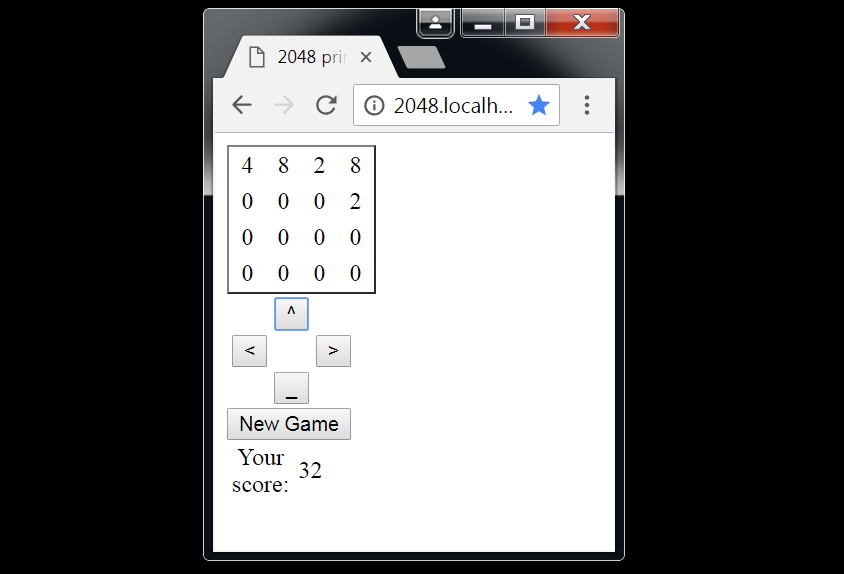
\includegraphics[width=\textwidth]{pictures/interface.png}}
\caption{Пользовательский интерфейс игры}
\label{move}
\end{figure}
В ситуации, когда следующий ход сделать невозможно, пользователю выводится сообщение \lk Game over!\rk.
\subsection{Архитектура приложения}
Приложение состоит из четырёх файлов - сама страница (index.html), файл стиля (stylesheet.css), функции, вызываемые страницей (application.js), логика, вызываемая из application (calc.js), функции вывода результата в html и запросов содержимого html (graphics.js).\\
Все скрипты имеют доступ к глобальным переменным Sum (текущий счёт) и GameoverFlag (булева переменная; в случае false игра завершена)
\begin{figure}[H]
\center{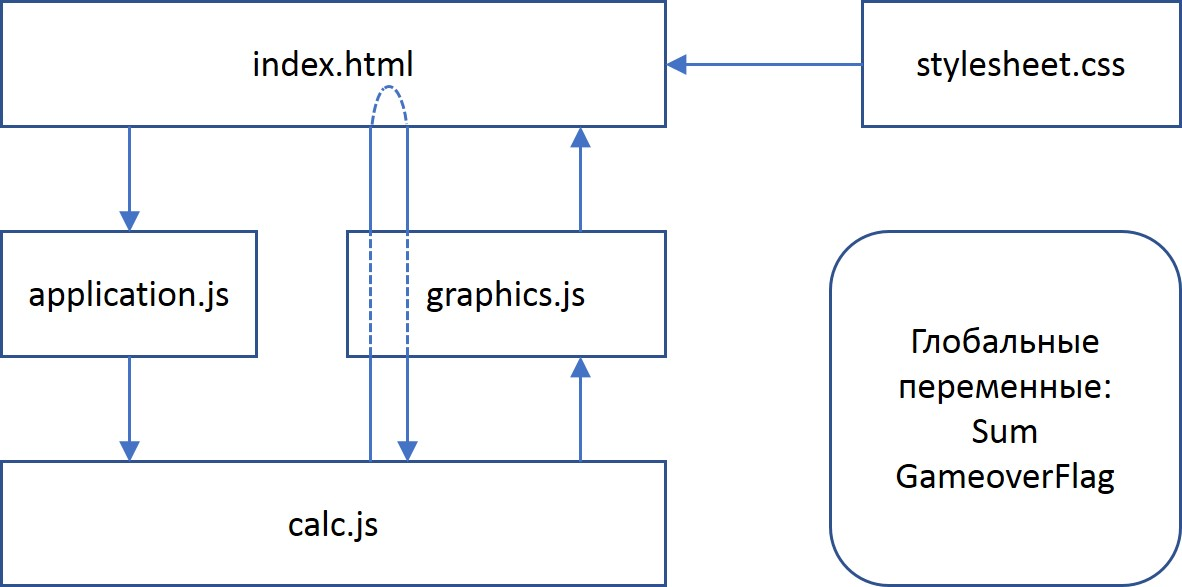
\includegraphics[width=\textwidth]{pictures/scheme.jpg}}
\caption{Схема взаимодействия файлов приложения}
\label{move}
\end{figure}
Файлы скриптов содержат следующие функции (везде A - двумерный массив $4\times4$, положение на игровом поле):
\begin{enumerate}
\item{application.js}
	\begin{enumerate}
	\item{init():} запускается, когда страница открывается или перезагружается
	\item{onrightpress():} запускается по нажатию экранной кнопки \lkвправо\rk. 			Аналогично onleftpress, ondownpress, onuppress.\\
	Если GameoverFlag равна true, совершает ход (вызывает move)
	\end{enumerate}
\item{calc.js}
	\begin{enumerate}
	\item{move(dir,A):} выводит на экран таблицу - результат хода из исходной 				позиции, заданной двумерным массивом A, в направлении dir (0-вправо, 1 - вниз, 2 		- влево, 3 - вверх) 
	\item{rotate(dir,A):} возвращает матрицу A, повёрнутую по часовой стрелке dir раз. 		Обёртка функций line\_rotate и angle\_rotate
	\item{rotateBack(dir,A):} возвращает матрицу A, повёрнутую против часовой 			стрелки dir раз
	\item{check(A):} возвращает булеву переменную. Если false, из положения A 			невозможно совершить ход ни в какую сторону
	\item{calc\_new\_pos(A):} возвращает двумерный массив - результат хода из положения A вправо
	\end{enumerate}
\item{graphics.js}
	\begin{enumerate}
	\item{draw(A):} заполняет таблицу - игровое поле в html значениями элементов A
	\item{gameover():} выводит на экран сообщение \lk Game over!\rk, устанавливает глобальную переменную GameoverFlag равной false
	\item{addPoints(points):} выводит на экран счёт (points)
	\item{getMatrix():} возвращает текущее состояние таблицы из html
	\end{enumerate}
\end{enumerate}
\subsection{Как осуществляется ход игрока}
\subsubsection{Общая схема работы программы}
При инициализации (init()) создаётся двумерный из нулей, в случайные места вставляются две двойки и результат выводится на экран. Пользователь может совершать ходы.\\
По нажатию экранной кнопки текуще положение считывается с экрана (getMatrix()) запускается move от этого положения и направления, соответствующего кнопке. Далее исполняются следующие команды:\\
\begin{lstlisting}
function move (dir, A) {
	console.log("func move");
	var A1 = rotate(dir,A);
	var A2=calc_new_pos(A1);
	var A3=rotateBack(dir,A2);
	addPoints(Sum);
	draw(A3);
	var flag = check(A3);
	if (flag == false) {
		gameover();
	}
} 
\end{lstlisting}
Пояснение к коду: 
\begin{enumerate}
\item{} Матрица поворачивается так, чтобы ход совершался направо;
\item{} Совершается ход направо, а также определяетсяо текущий счёт (изменяется глобальная переменная Sum);
\item{} Матрица поворачивается обратно;
\item{} Счёт выводится на экран;
\item{} Матрица выводится на экран (в игровое поле);
\item{} Проверяется, возможен ли следующий ход;
\item{} Если следующий ход невозможен, запускается функция gameover.
\end{enumerate}
Функция Gameover, как было сказано выше, изменяет глобальную переменную GameoverFlag и оповещает пользователя о том, что игра закончена:
\begin{lstlisting}
function gameover(){
	afterScoreText.innerHTML='Game over!';
	GameoverFlag=true;
}
\end{lstlisting}
\subsubsection{Функции сдвига и заполнения случайных клеток таблицы}
Все функции обёрнуты в функцию calc\_new\_pos(A), внутри которой для прерывания ссылки на A матрице A1 поэлементно присваиваются значения A, после чего вызывается shiftAndClap(A1).\\
Функция ShiftAndClap перебирает справа налево элементы массива и соединяет элементы одного номинала, присваивая удвоенную стоимость элементу справа.После этого осуществляется функция сдвига shift.\\
Функция сдвига shift(B) осуществляет перебор с четвертого элемента первой строки и двигается справа налево сверху вниз, находит элемент, справа от которого стоит ноль и меняет их местами. Если таковой элемент найден и сдвинут, возвращается в конец строчки и переходит на следующую только тогда, когда все элементы сдвинуты вправо\\
Функция добавления в случайное место 2 или 4 -  addRandNum. Сначала идет генерация 2 или 4 с вероятностью 25/75 соответственно. После этого идет перебор всех элементов массива и запоминание мест нулей в массивы placeOfNulli и placeOfNullj.Далее случайным образом выбирается место и присваивается сгенерированное число.\\
\subsubsection{Функции поворота матрицы}
В ходе работы над проектом наша группа приняла решение написать только одну функцию сдвига по направлению влево, вместо того чтобы писать функции сдвига для каждого из направлений. Данное решение привело к необходимости вращать матрицу до и после осуществления сдвига. Ниже приведена схема сдвигов, которая наглядно демонстрирует алгоритм поворота матрицы в зависимости от направления сдвига:
\begin{figure}[H]
\center{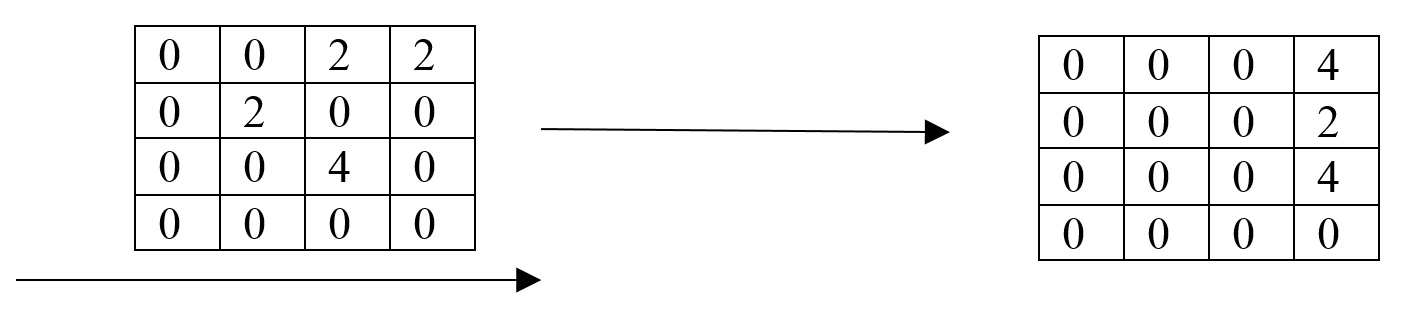
\includegraphics[width=\textwidth]{pictures/matrixMove2.jpg}}
\caption{Сдвиг вправо}
\label{move}
\end{figure}
Сдвиг вправо - базовый случай, поворот не требуется. К нему сводятся остальные путём поворота.
\begin{figure}[H]
\center{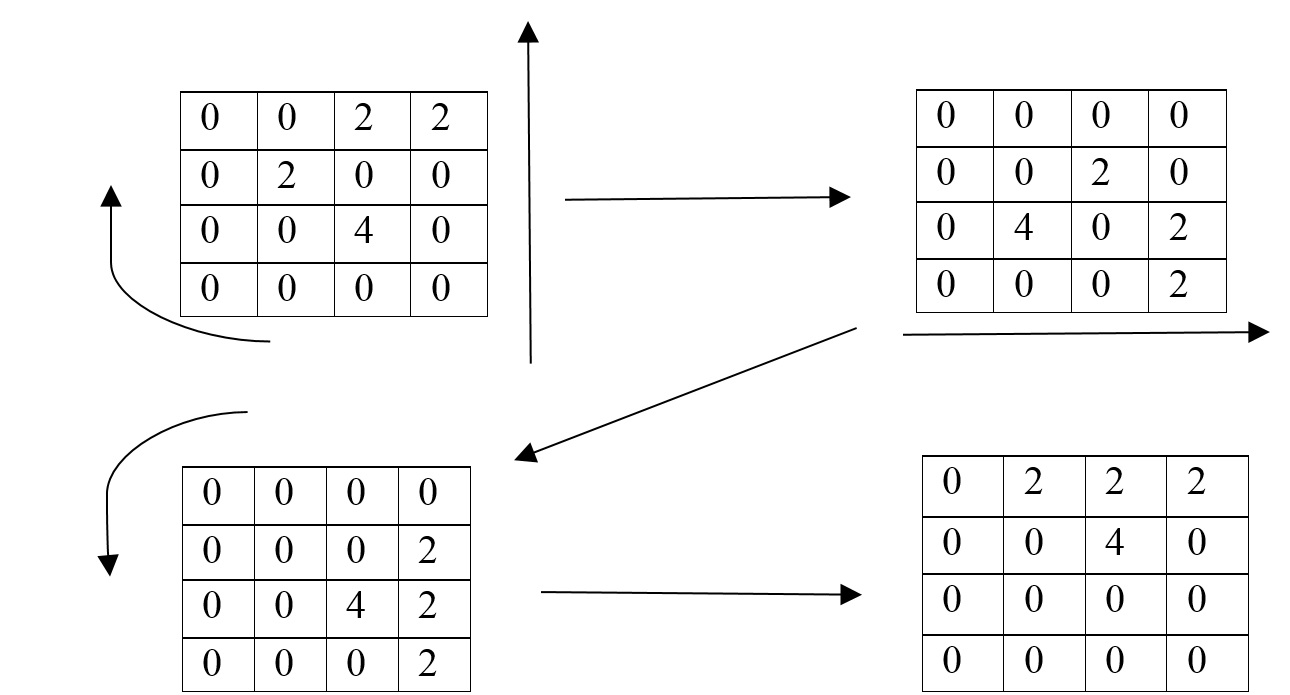
\includegraphics[width=\textwidth]{pictures/matrixRotate2.jpg}}
\caption{Сдвиг вверх путём поворота и сдвига вправо}
\label{rotate}
\end{figure}
Приведём код этих поворотов:
\begin{enumerate}
\item{} разворот на 180 градусов для сдвига влево:\\

\begin{lstlisting}
function line_rotate(A){
   //required for turn on 180 degrees
   var A_rotate=[];
   for(var i = 0; i < 4; i++){
      A_rotate.push([]);
      for(var p = 0; p < 4; p++){
         A_rotate[i].push(A[i][3-p]);
      }
   }
   return A_rotate;
}
\end{lstlisting}
Исполнение данной операции осуществляется за счёт вложенного цикла, что позволяет переписать каждый из вложенных массивов в обратном порядке.

\item{} Разворот по или против часовой стрелки:\\
\begin{lstlisting}
function angle_rotate(A,dir){
   var A_rotate=[]
   if (dir == 1){
      /*first turn for "up", second for "down"*/
     for(var i = 0; i < 4; i++){
        A_rotate.push([])
         for(var p = 0; p < 4; p++){
           A_rotate.push(A[3-p][i])
         }
      }
   }
   if (dir == 3){ 
      /*first turn for "up", second for "down"*/
      for(var i = 0; i < 4; i++){
         A_rotate.push([])
         for(var p = 0; p < 4; p++){
            A_rotate.push(A[p][3-i])
         }
      }
   }
   return A_rotate
}
\end{lstlisting}
Данная функция проверяет в каком направлении следует вращать матрицу и в зависимости от этого переписывает новую матрицу построчно с помощью вложенного цикла.
\end{enumerate}
\subsubsection{Функция проверки возможности кода check}
Матрица A сравнивается с другой, полученной из A сдвигом направо. Если есть хоть один элемент, отличный от эл-та в матрице A - значит, ход возможен. Далее A поворачивается по часовой стрелке и процесс повторяется. Если даже после треьего поворота нет ни одной позиции, в которой матрица после сдвига была бы отличной от исходной, возвращается false (нет возможных ходов).\\
\begin{lstlisting}
function check(A){
	var T=null;
	var flag=false;
	for (var i=0; i<4; i++){
		T=calc_new_pos(A);
		for (var j=0; j<4; j++){
			for (var k=0; k<4; k++){
				if(T[j][k]!=A[j][k]){
					flag=true;
					return flag;
				}
			}
		}
		A=rotate(1,A);
	}
	return flag; //false=>gameover
}
\end{lstlisting}
\section{Распределение работ}
Работа над проектом была распределена следующим образом:
\begin{itemize}
\item{Зуев В.:} Графический интерфейс и архитектура приложения\\
Файлы - index.html, stylesheet.css, graphics.js, application.js
\item{Комаров Г.:} Алгоритм вычисления следующей позиции после хода игрока и алгоритм вычисления текущего счёта игры\\
Файл calc.js (функция calc\_new\_pos)
\item{Великов М.:} Вспомогательные алгоритмы для задания позиции и проверка возможности совершить ход.\\
Файл calc.js (функции rotate, rotateBack, check)
\end{itemize}
Все авторы принимали участие в написании отчёта.
\section{Результаты}
Создано Web-приложение - игра. Поставленные задачи (игра по правилам, вывод счёта, завершение игры) выполнены.\\
Исходный код проекта можно найти по адресу \href{https://github.com/zuevval/2048}{github.com/zuevval/2048}.\\
Работу приложения можно посмотреть на сайте \href{http://2048.timefwd.ru}{2048.timefwd.ru}.
\section{Заключение}
Объектно-ориентированный язык Javascript позволяет в связке с языком разметки HTML быстро создавать графический интерфейс браузерных приложений. Встроенный в браузер (например, в  Google Chrome) отладчик предоставляет широкие возможности для оптимизации кода и устранения ошибок. Впрочем, необходимо учитывать особенности задания переменных через значения других - часто вместо создания независимой переменной новое имя содержит лишь ссылку на существующий объект.\\
Возможностей Javascript хватило для написания полноценного web-\-при\-ло\-жения - игры \lk2048\rk. Проект доведён до завершённого состояния, но может быть улучшен: планируется изменить дизайн (например, добавить анимацию сдвига цифр на поле методами Javascript) и добавить серверную часть для хранения рекордов.
\end{document}